\subsection{\auspice\ vs. managed DNS providers}
\label{sec:managed}

%In DNS terminology, an \auspice\ name server provides the functionality of an authoritative name server -- it keeps the most up to date  name-to-address mapping of a host. 

Having analyzed a synthetic workload dominated by mobile device names, we next evaluate how \auspice\ compares to commercial managed DNS providers in serving their customers' (mostly static) domain names.  These providers such as UltraDNS, DynDNS, and DNSMadeEasy \cite{ultradns, dyndns, dnsmadeeasy} offer a geo-replicated authoritative DNS service and are widely used by enterprises today (e.g., DynDNS provides DNS service for Twitter).

%Similar to the role of a replica of a name record in \auspice, managed DNS providers such as UltraDNS, DynDNS, and DNSMadeEasy \cite{ultradns, dyndns, dnsmadeeasy}  offer a geo-replicated authoritative DNS service for domain names.%\footnote{DNS Services such as Open DNS \cite{opendns}, and Google DNS \cite{googledns} maintain local name servers that store cached name records  and therefore are not managed DNS services.}

%Note that Open DNS \cite{opendns}, Google DNS \cite{googledns} and other similar services which offer name lookup service to their users  maintain local name servers that store cached name records  and therefore are not managed DNS services. 


%Managed DNS providers such as UltraDNS, DynDNS, and DNSMadeEasy \cite{ultradns, dyndns, dnsmadeeasy} offer a geo-replicated authoritative DNS service similar to \auspice.
%Managed DNS providers differ from services such as Open DNS \cite{opendns}  and Google DNS \cite{googledns} as the former maintain authoritative name servers for domain names of their customers and the latter maintain local name servers that store cached name records. 



%Managed DNS providers \cite{ultradns,dyndns,dnsmadeeasy} offer a geo-replicated DNS service, and are commonly purchased by enterprises today. This section compares \auspice\ to managed DNS providers in terms of lookup and update latencies. 

\textbf{Lookup latency:}  
We compare \auspice\ to UltraDNS for a workload of lookup requests for  domain names serviced by the provider. 
%This experiment compares lookup latencies for \auspice\ and a leading managed DNS provider. 
%Our workload consists of lookups for  domain names serviced by the provider.  
We identify 316 domain names among top-10K Alexa websites \cite{alexa} serviced by this provider. 
The geo-distribution of lookups for each name is determined from the Alexa dataset \cite{alexa}.
For each name, we measure performance for 1000 lookups across 100 PlanetLab nodes. 
We ensure that lookups are served from the name servers maintained by the provider by requesting the address for a new random sub-domain name each time, e.g,, xyz.google.com instead of google.com. 
This name is unlikely to be cached and requires an authoritative name server lookup.
\auspice\ name servers are deployed on 80 PlanetLab locations while the managed DNS has 16 known locations of server deployments \cite{dnscompare}.  
For an even comparison between \auspice\ and the provider, we limit the maximum number of replicas/name for \auspice\ to 5, which is less than one-third the number of locations of the provider \cite{dnscompare}.  
%The geo-distribution of lookups for each domain name is determined based on the Alexa dataset \cite{alexa}.




%The list of MDNS deployments is obtained from this report \cite{dnscompare}. The median and maximum different between \auspice\ name server and the corresponding MDNS deployment was X miles and Y miles respectively.  


 
%This technique has also been used by another study \cite{dnscompare} to measure latencies to authoritative name servers.

\begin{table}[h]
\centering
\small{
\begin{tabular}{l c  c }
  & \textbf{\auspice}  & \textbf{UltraDNS}  \\ \hline
Number of replicas & 5 & 16  \\ \hline
Median Lookup Latency & 45 & 40 \\ \hline
Mean Lookup Latency & 74 & 72\\ \hline
\end{tabular}
}
\caption{\auspice\ has latencies comparable to a managed DNS provider with less than one-third replica locations.}
\label{tab:manageddns}
\end{table}




%\begin{table}[h]
%\centering
%\small{
%\begin{tabular}{l c  c  c}
%{\bf Lookup latency (ms)  $\rightarrow$} & {\bf Median}  & \textbf{Mean} & {\bf 95-\%ile}  \\ \hline
%\auspice\ &	45  & 74 & 246 \\ \hline
%Managed DNS	 & 40   & 72 & 259 \\ \hline
%\end{tabular}
%}
%\caption{\auspice\ has latencies comparable  to a managed DNS provider with less than one-third replica locations.}
%\vspace{-0.1in}
%\label{tab:manageddns}
%\end{table}



%Figure \ref{fig:manageddns} shows the CDF of the median lookup latencies across names for \auspice\ and for the managed DNS provider. The median value of the distribution in Figure \ref{fig:manageddns} is 45 ms for  \auspice\ and 40 ms for the managed DNS provider. 
Table \ref{tab:manageddns} shows median lookup latencies across names for \auspice\ and for the managed DNS provider.
\auspice\ performs within 11\% of the managed DNS provider for all latency metrics. 
While \auspice\ creates less than one-third replicas as the managed DNS provider, it places them considering the geo-distribution of demand. 
Due to its placement strategy, \auspice\ achieves  similar latency with smaller cost of updates.
% \auspice\ has a comparable latency to the managed DNS provider even with less than one-third the number of replicas for every name record as the managed DNS provider.  
%Due to a locality-aware placement,
 This experiment shows that \auspice\ provides  latencies comparable to the state-of-the-art DNS solutions with much smaller update costs due to a judicious choice of replica locations. 

%This experiment shows that due to the to the geo-locality of requests for today's domain  names, a locality-aware placement reduces update costs.



\textbf{Update propagation latency:} To measure update propagation latencies, we purchase DNS service from three providers for separate domain names.  All providers replicate a name at 5 locations across US and Europe for the services we purchased. We issue address updates for the domain name serviced by that provider and then immediately start lookups to the authoritative name servers for our domain name.
These authoritative name servers can be queried only via an anycast IP address, i.e., servers at different locations advertise the same externally visible IP address. Therefore, to maximize the number of provider locations queried, we send queries from 50 random PlanetLab nodes. From each location, we periodically send queries until all authoritative name server replicas return the updated address.  The update propagation latency at a node is the time between when the node starts sending lookup to when it receives the updated address. The latency of an update is the the maximum update latency measured at any of the nodes. We measure latency of 100 updates for each provider.
 %is time difference between when we update an address and when the node gets the updated address. 

To measure update latencies for \auspice, we replicate 1000 names at a fixed number of PlanetLab nodes across US and Europe. The number of nodes is chosen to be 5, 10, and 20 across three experiments. A client sends an update to the nearest node and waits for update confirmation messages from all replicas. The latency of an update is the time difference between when the client sent an update and when it received the update confirmation message from all replicas (an upper bound on the update propagation latency).  We show the distribution of measured update latencies for \auspice\ and for three managed DNS providers in Figure \ref{fig:manageddnsupdate}.   

%The update latency for \auspice\ is shown based on the experiment in Section \ref{sec:lowload};  we select names replicated at 5 locations or more, because 

%We issue address updates for the domain name serviced by that provider, and simultaneously start lookups to the provider's name servers from 50 PlanetLab nodes until the updated address is returned by all the name servers. 
%We issue address updates  for DNSMadeEasy using a REST-based API and for UltraDNS using a web portal.


%\begin{table}[h]
%\centering
%\small{
%\begin{tabular}{p{1.5cm}p{1cm}p{1cm}p{1cm}p{1cm}}
%{\bf Update latency(s)} & {\auspice}  & Managed DNS 1 & Managed DNS 2  & Managed DNS 3 \\ \hline
%\textbf{Median} &	0.3 & 1.4 & 1.5 & 25.0 \\ \hline
%\textbf{95-\%ile}	& 0.6 & 5.3   & 3.0 & 99.0 \\ \hline
%\end{tabular}
%}
%\caption{\auspice' update latencies are smaller than managed DNS providers for equal or more replica locations.}
%\vspace{-0.1in}
%\label{tab:manageddnsupdate}
%\end{table}

%
%\begin{figure}
%\centering
%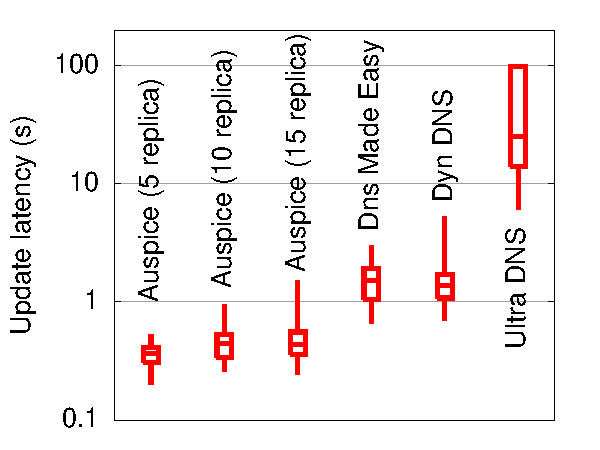
\includegraphics[scale=0.55]{auspice/graph/newgraphs/managed-update.pdf}
%\vspace{-0.1in}
%\caption{Median  update latency of \auspice\ for updating replicas at 5 locations is  1.0 sec to 24.7 sec lower than three managed DNS providers. Values shown are 5, 25, 50, 75,  and 95 percentiles.}
%\vspace{-0.2in}
%\label{fig:manageddnsupdate}
%\end{figure}

\auspice\ provide lower update propagation latencies than all three providers for an equal or greater number of replica locations for names.  It is not clear to us why UltraDNS's update latencies are an order of magnitude higher than global propagation delays\footnote{They tend to not be forthcoming with proprietary internal details.}. This finding is consistent with a recent study \cite{dnscompare} that has shown latencies of up to tens of seconds for these providers. 

%\vspace{-0.15in}
\eat{
\subsection{[Simulation]  Sensitivity analysis}
\label{sec:sensitivity}

We analyze the sensitivity of \auspice's benefits to the workload parameters used in $\S$\ref{sec:comparison}. In order to be able to explore a wider range of parameters and scales, we use a custom simulator that simulates round-trip latency, loss, and server load-vs-response time behavior as measured on PlanetLab. We have verified \cite{techreportAuspice} that the median latencies for all schemes in the simulator are within 8\% of that on PlanetLab for the experiment in $\S$\ref{sec:comparison}.   Experiments here use 10K nameservers, 2K local nameservers, 10K service names, and 100K device names. 


%\auspice\ consistently gives lower lookup latencies, and its performance is robust to variations in these workload parameters.

%We present sensitivity analysis of parameters in our synthetic workload for device names: geo-locality, ratio of lookups to updates, and the distribution of lookup rates of names.  Overall, we find that our prior results are robust to variation in values of these parameters. 
%Our results show that \auspice\ consistently provides better performance for a broad range of these workload parameters. 



%TBD: What is the ratio of lookups to updates for device names? What is the ratio of lookups for device names to lookups for service names?





%\begin{figure*}[ht]
%\subfigure[Geo-locality]{\label{fig:varylocality}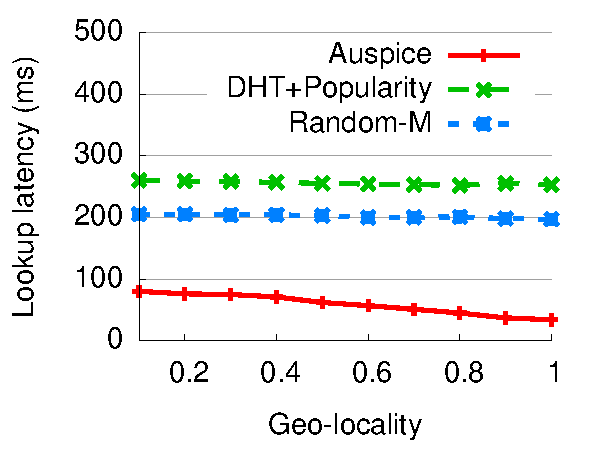
\includegraphics[scale=0.4]{graph/medianlatencyVSlocality.pdf}}
%\subfigure[Lookup rate distribution]{\label{fig:lookupdis}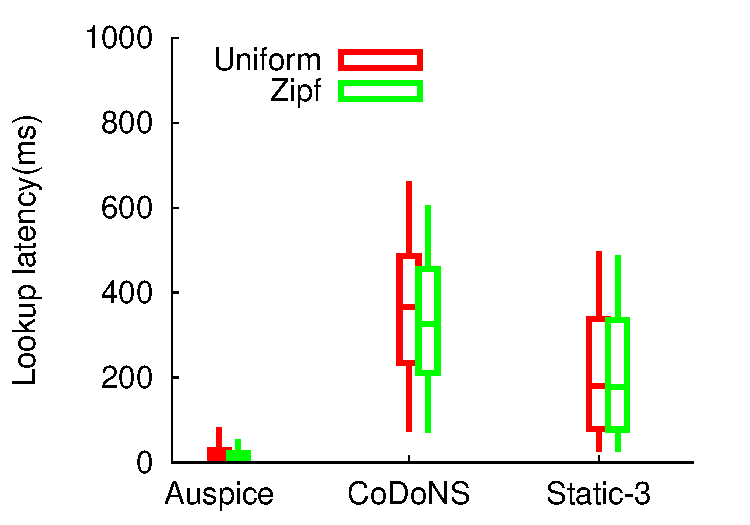
\includegraphics[scale=0.4]{graph/newgraphs/lookupdis.pdf}}
%\subfigure[Ratio of device names to service names]{\label{fig:varymobile}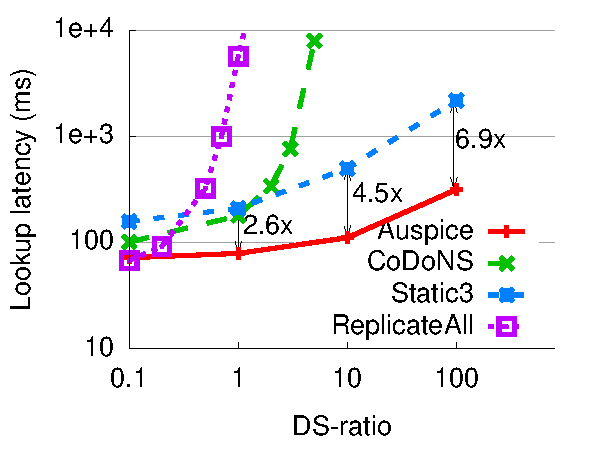
\includegraphics[scale=0.4]{graph/medianlatencyVSnummobile.pdf}}
%\subfigure[Lookup-to-update ratio]{\label{fig:readwriteratio}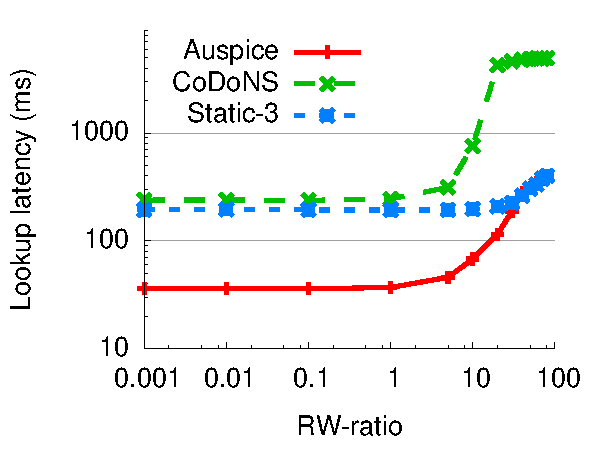
\includegraphics[scale=0.4]{graph/readwriteratio.pdf}}
%\subfigure[Update cost]{\label{fig:updatebw}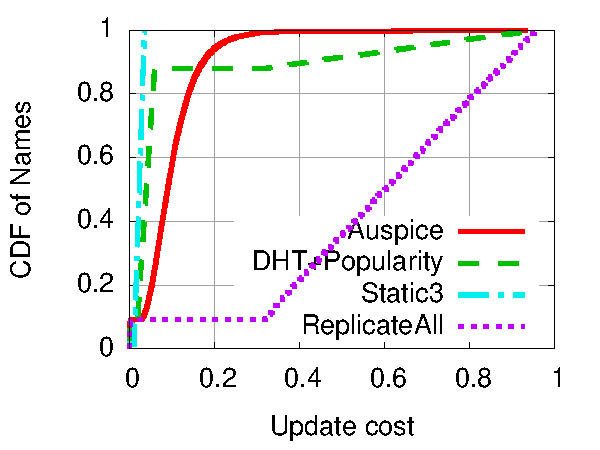
\includegraphics[scale=0.55]{graph/newgraphs/cdf-update-cost.pdf}}
%\vspace{-0.15in}
%\caption{[Simulator] Workload sensitivity. (a) \auspice\ gives 2$\times$ to 5$\times$  lower latencies across all locality levels. (b)  \auspice\ gives greater latency gains over \staticthree\ as the number of device names increases in  the workload.  (c) \auspice\ has lower latencies for both lookup- and update- dominated workloads. \replicateall\ is unsustainable due to high update costs and is not shown.}
%\vspace{-0.15in}
%\label{fig:lookupupdate}
%\end{figure*}

%
%\begin{figure}[t]
%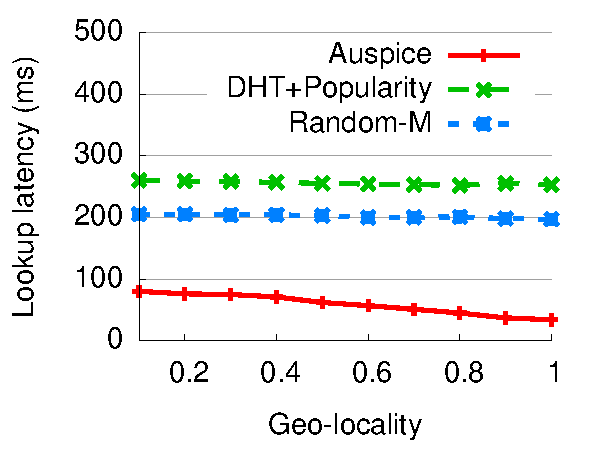
\includegraphics[scale=0.5]{graph/medianlatencyVSlocality.pdf}
%\vspace{-0.1in}
%\caption{[Simulator] Workload sensitivity. \auspice\ gives 2$\times$ to 5$\times$  lower latencies across all locality levels.}
%\label{fig:varylocality}
%\vspace{-0.1in}
%\end{figure}

%  For a read-dominated workload (RW-ratio = 10), \auspice\ has 2.95$\times$ lower latency than \staticthree.

%
%\begin{figure}
%\centering
%
%\vspace{-0.1in}
%\caption{[Simulator] \auspice\ outperforms other schemes by 2$\times$ to 5$\times$  across all locality levels. \replicateall\ has  100\% request failure rate  (not shown).}
%\label{fig:varylocality}
%\vspace{-0.1in}
%\end{figure}
%
%
%\begin{figure}
%\centering
%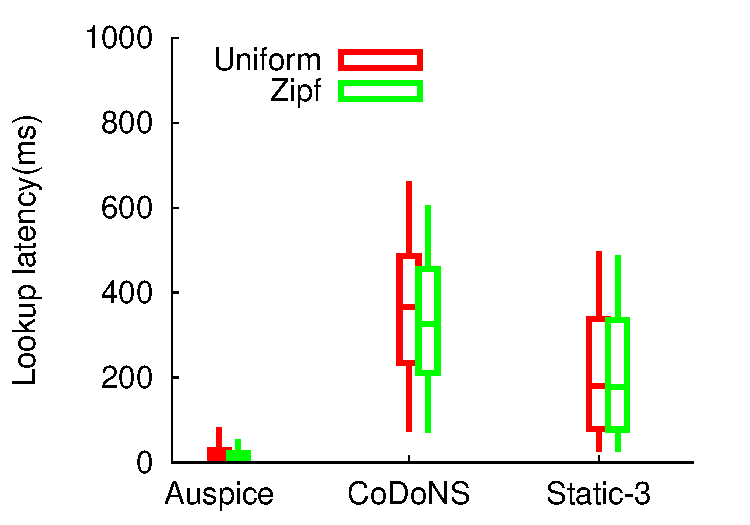
\includegraphics[scale=0.4]{graph/newgraphs/lookupdis.pdf}
%\vspace{-0.1in}
%\caption{[Simulator] Distribution of lookup rates.}
%\label{fig:lookupdis}
%\vspace{-0.1in}
%\end{figure}
%
%
%\begin{figure}
%\centering
%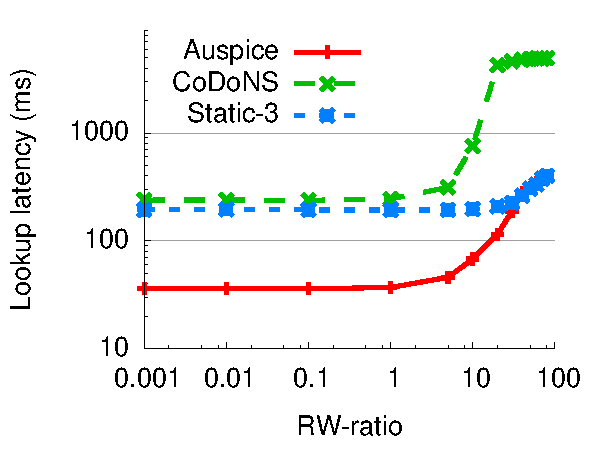
\includegraphics[scale=0.5]{graph/readwriteratio.pdf}
%\vspace{-0.1in}
%\caption{[Simulator] Ratio of lookups to updates for device names. For a lookup-dominated workload (RW-ratio = 10), \auspice\ has 2.95$\times$ lower latency than \staticthree.  \replicateall\ has 100\% request failure rate (not shown).}
%\label{fig:readwriteratio}
%\vspace{-0.1in}
%\end{figure}


\textbf{Geo-locality:}  Figure \ref{fig:varylocality} compares the latency for workloads with varying levels of geo-locality.
Both \staticthree\ and \codons\ are choose replica locations randomly, and therefore their latency remains the same irrespective of workload locality. But \auspice\ can achieve better latencies  as the geo-locality in the workload increases. Even in a workload with no locality ($g=0.1$),   \auspice\ outperforms \staticthree\ by 2$\times$ because it creates more than three replicas for each name,  and outperforms \codons\ by $4\times$  because it redirects requests to the closest replica of a name unlike \codons.

\textbf{Ratio of device names to service names:} We also evaluate schemes for workloads with different ratios of device names to service names.
We fix the number of service names to be 10K and vary the number of device names between 1000 to 1,000,000.
%\replicateall\  saturates server capacity for a workload with  DS-ratio = 1 due to high update costs. 
\auspice\  can accommodate workload with up 1M device names (\replicateall\ can support at most 1K device names) and provides up to 6.9$\times$ lower latencies over \staticthree\  across for all ratios of service to device names.

% up to 100  as it minimizes the update cost for device names. 
% \auspice\ has up to 6.9$\times$ lower latency than \staticthree\ and \codons\ due to itts locality-aware design,

\textbf{Lookup-to-update ratio:} We vary the ratio of lookups to updates, termed as \emph{RW-ratio}, by increasing the number of lookups but keeping the number of updates fixed. \auspice\ provides up to 2.95$\times$ lower latencies than \codons\ and \staticthree\ for both write-dominated workload (RW-ratio $<$ 1) as well as read-dominated workloads (RW-ratios  $>$ 1). As RW-ratios increase beyond 1,  \auspice\ handles the increase in number of lookups  by decreasing the replication parameter $\beta$ (refer to Eq. \ref{eq:mu}).
}
\subsection{Scalability}
\label{sec:scalability}

\begin{figure}[t]
\centering
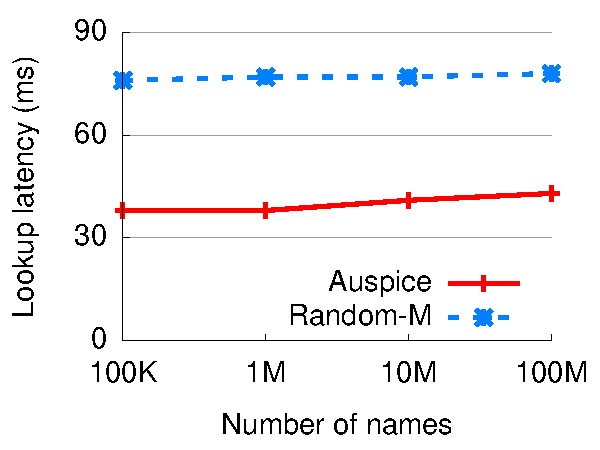
\includegraphics[scale=0.6]{auspice/graph/newgraphs/scalability.pdf}
\caption{\auspice's consistently gives close to 2$\times$ lower latencies for workloads with 100K-100M names.}
\vspace{-0.2in}
\label{fig:scalability}
\end{figure}

%How will \auspice\ perform at a scale of 10 billion mobile devices? 
To evaluate \auspice's key design traits at very high scales, we evaluate \auspice\ on workloads with 100K-100M device names.  We use a testbed of 200 Amazon EC2 instances, 100 each for nameservers and local nameservers respectively. We emulate wide-area latencies among servers as in the experiments in Section \ref{sec:lookup}. The experiment with a workload of 100M names included 1 billion requests with an equal number of lookups and updates sent over a 4 hour duration. Experiments with lesser number of names proportionally scale down the number of requests and the  duration.  
%As our focus is on evaluating the performance of \auspice's data plane, \auspice\ pre-computes the placement at the start of the experiment based on prior knowledge of the workload. Local name servers are also aware of the precomputed placement and they send requests directly to the active replicas in this experiment. Evaluating  \auspice's control plane performance at larger scales is part of our ongoing work.

Figure \ref{fig:scalability} shows that median lookup latency for Auspice and for \staticthree. We find that \auspice\ consistently gives close to 2$\times$ lower latency than \staticthree\ across all four workloads. 
\auspice's performance is consistent across workloads because its placement strategy ensures a similar distribution of load across name servers independent of the number of names in the workload.
Given that \auspice\ shows similar relative performance across 4 orders of magnitude of variation in the number of names, we expect these properties to persist at higher scales. Intuitively, this result is not surprising: the core of \auspice's replica placement engine is designed to make between M (the minimum required for fault-tolerance) and N (the total number of nameservers) replicas and use all available resources for intelligent replication. Group changes, although nontrivial in design, do not impose a high control overhead.



%\textbf{Lookup rate distribution:} We evaluate performance for (a) Zipf  and (b) uniform popularity distribution of  lookup rates of users The mean lookup rates are same for both distributions. As Figure \ref{fig:lookupdis} shows, the lookup latency of all schemes are nearly equal for the two distributions.  The performance of \staticthree\ is unchanged because its replica placement is fixed. \codons\ sees high latency for both distributions because its design replicates most names at a small number of locations for both distributions (a small percent of highly popular names are replicated at larger number of locations). The median lookup rates are smaller for Zipf-distribution compared to uniform distribution, i.e., a typical name has a smaller read-to-write ratio for Zipf-distritbution compared to uniform distribution . Hence, \auspice\ create less number of replicas for most names. Still, the number of replicas for names is sufficiently high in this experiment to keep the lookup latency nearly the same. 

%The slightly better latencies for \auspice\ for the Zipf-distribtuion are because of  highly popularity names see a improv

%\codons\ decides number of replicas only based on popularity ranking of a name and not on the value of the lookup rates, and hence its distribution of the number of replicas of names remains unchanged due to a change in the popularity distribution. 

%The performance of \codons\ and \staticthree\ are unchanged as they 

%Across experiments, we change the distribution of lookup rates of users keeping the average lookup rate unchanged.  Figure X shows the results. 

%This experiment suggests that our results from prior experiments are likely to hold irrespective of the specific distribution of lookup rates of users.


\eat{
\begin{figure}
\centering
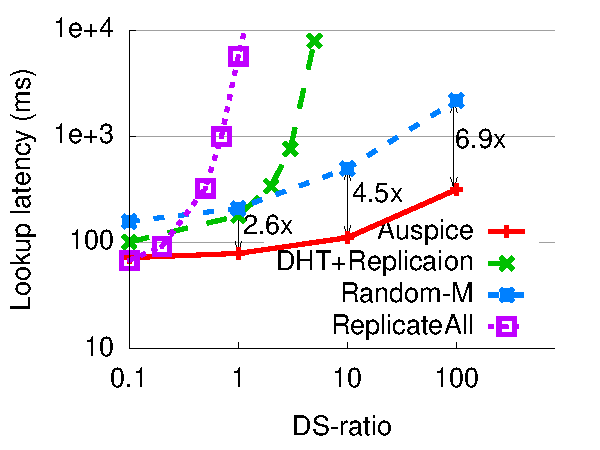
\includegraphics[scale=0.5]{auspice/graph/medianlatencyVSnummobile.pdf}
\vspace{-0.1in}
\caption{[Simulator] \auspice\ gives greater latency gains over \staticthree\ as the number of device names increases in  the workload.}
\label{fig:varymobile}
\end{figure}

\textbf{Ratio of device names to service names:} This experiment evaluates schemes for workloads with different ratios of device names to service names, called \emph{DS-ratio} for short.
We fix the number of service names to be 10K and vary the number of device names between 1000 to 1,000,000.
Figure \ref{fig:varymobile} presents our results.
\replicateall\  saturates server capacity for a workload with  DS-ratio = 1 due to high update costs. 
\auspice\  supports workloads with DS-ratio up to 100  as it minimizes the update cost for device names. 
Due to its locality-aware design, \auspice\ has  2.6$\times$, 4.5$\times$ and 6.9$\times$ lower latency than \staticthree\ when DS-ratios are 1, 10 and 100 respectively. 

\textcolor{blue}{
 \codons's latency increases more sharply than \auspice\ and \staticthree\  on increasing the number of device names.  
\codons\ creates  a greater number of replicas for device names than \auspice\ and \staticthree, which increases update cost and, as a result, the lookup latency for \codons.
For example, for a workload with DS-ratio = 2  and an average hop count of 2.0, \codons\ creates an average of 24 replicas/name compared to three replicas/name for \staticthree. We experimented with average hop-count values as high as 10, but the number of replicas did not reduce further.}
}
%, while using the recommended value of 16 for Pastry DHT's base parameter \cite{codons-paper}. 
%To reduce the number of replicas for \codons, we experimented with average hop count values up to 20 while using the recommended value of 16 for Pastry DHT's base parameter \cite{codons-paper}. But \codons\  still created more replicas  than \staticthree\ and \auspice.

% TBD: Figure 8 (DS-ratio) and Figure 9 (Geo-locality) are inconsistent. Our default DS-ratio is 10. In figure 8, Codons has higher latency than Static3 for DS-ratio = 10, but in figure 9 at Geo-locality of 1, Codons has lower latency than Static3 for  DS-ratio = 10.



%In earlier experiments, 90\% requests for a device name show a strong geo-locality and 10\% requests originate from random  locations. 
%We vary the workload geo-locality by changing the fraction of requests that originate from random  locations.  A \emph{geo-locality} of $p$ means (1-$p$) fraction of requests originate from random  locations.


\eat{
\textbf{Ratio of lookups to updates (vary the write rate:} We vary the ratio of lookups to updates, termed as \emph{RW-ratio}, by varying the number of updates in the workload, but keeping the number of lookups fixed. Figure \ref{fig:readwriteratio} shows the results. As the RW-ratio decreases, the update rates are smaller, which reduces load on the name servers. \auspice\ uses the extra available capacity at the name servers to create more replicas closer to the pockets of demand for the name. As a result, \auspice\ sees a better latency compared to \codons\ and \staticthree\ for workload with higher RW-ratios. An interpretation of this result is that \auspice\ consistently gives better performance for a wide range of mobility rates of users. 
}


%\textbf{Lookup-to-update ratio:} We vary the ratio of lookups to updates, termed as \emph{RW-ratio}, by increasing the number of lookups in the workload, but keeping the number of updates fixed. Figure \ref{fig:readwriteratio} shows that \auspice\ provides lower latencies for both write-dominated workload (RW-ratio $<$ 1) as well as read-dominated workloads (RW-ratios  $>$ 1). As RW-ratios increase beyond 1,  \auspice\ handles the increase in number of lookups in the workload by decreasing the replication parameter $\beta$ (refer to Equation \ref{eq:mu}). Lower $\beta$ values reduce number of replicas and hence the update costs for \auspice, which helps \auspice\ accommodate workloads with  RW-ratio $>$ 1. Reduced number of replicas increases  lookup latency of \auspice, but still \auspice\  has 2.95$\times$ lower latency than \staticthree\  for RW-ratio = 10. 



%At RW-ratio $>$ 5, \codons's latency is higher than both \staticthree\ and \auspice. This is because  \codons\ creates identical number and location of replicas for every name at all RW-ratios $>$ 1; tuning the hop-count parameter does not reduce the number of replicas further. Thus, \codons\ update cost remains the same, but increase in RW-ratio adds to the load-induced latency at name servers, which reflects in increased lookup latency for \codons.




\eat{

\begin{figure}
\centering
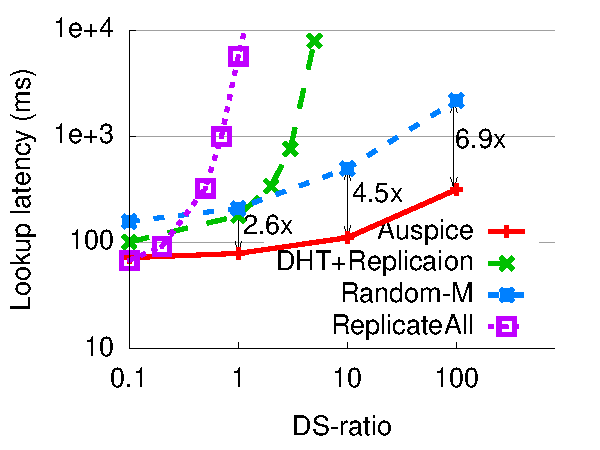
\includegraphics[scale=0.5]{auspice/graph/medianlatencyVSnummobile.pdf}
\vspace{-0.1in}
\caption{[Simulator] \auspice\ gives greater latency gains over \staticthree\ as the number of device names increases in  the workload.}
\label{fig:varymobile}
\end{figure}


\textbf{Ratio of device names to service names:} This experiment evaluates schemes for workloads with different ratios of device names to service names, called \emph{DS-ratio} for short.
We fix the number of service names to be 10K and vary the number of device names between 1000 to 1,000,000.
Figure \ref{fig:varymobile} presents our results.
\replicateall\  saturates server capacity for a workload with  DS-ratio = 1 due to high update costs. 
\auspice\  supports workloads with DS-ratio up to 100  as it minimizes the update cost for device names. 
Due to its locality-aware design, \auspice\ has  2.6$\times$, 4.5$\times$ and 6.9$\times$ lower latency than \staticthree\ when DS-ratios are 1, 10 and 100 respectively. 

 \codons's latency increases more sharply than \auspice\ and \staticthree\  on increasing the number of device names.  
\codons\ creates  a greater number of replicas for device names than \auspice\ and \staticthree, which increases update cost and, as a result, the lookup latency for \codons.
For example, for a workload with DS-ratio = 2  and an average hop count of 2.0, \codons\ creates an average of 24 replicas/name compared to three replicas/name for \staticthree. We experimented with average hop-count values as high as 10, but the number of replicas did not reduce further.
}



\eat{
\subsubsection{Scalability analysis}

Figure \ref{fig:scalability} evaluates the scalability of \auspice. In this experiment, we increase the number of name servers from 100 and 100,000, while keeping the total system capacity to be constant. The figure shows that \auspice\ is able to achieve the lowest latency while at the same time scales well to increasing number of servers. In contrast, \replicateall\ and \codons\ have poor scalability performance and saturate quickly.

To illustrate the scalability benefits of \auspice, consider a back of the envelope calculation based on the maintenance cost (\$\$) and network bandwidth needed for record update. Assume the number of servers increases by one order of magnitude (e.g., from 100 to 1000) while the total system capacity remains the same. Then \codons\ and  \replicateall\ will incur the same order of magnitude increase in terms of server maintenance cost and update bandwidth, because they replicate names at one order of magnitude more replicas and simply ignore the capacity constraint of the whole system. However, \auspice\ replicate names making sure that the aggregate system load is below a threshold of the capacity(refer \S 3.2.1), therefore it does incur additional maintenance cost and update bandwidth.

\begin{figure}
\centering
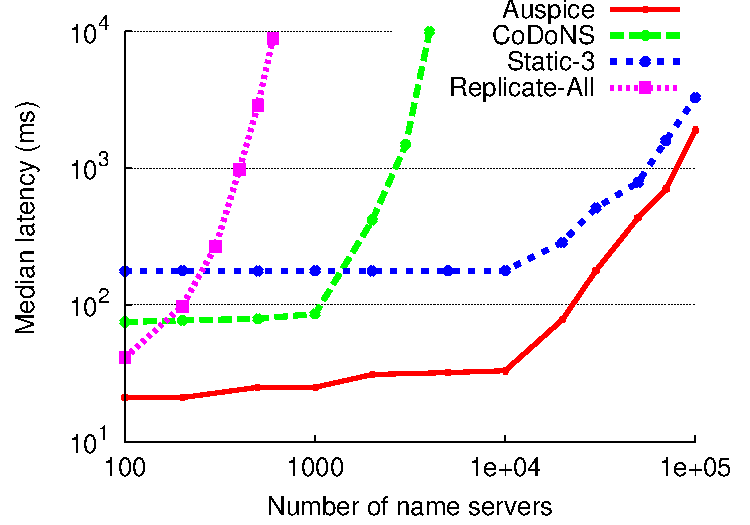
\includegraphics[scale=0.5]{auspice/graph/medianlatencyVSnumns.pdf}
\vspace{-0.1in}
\caption{[Simulator] \auspice\ scales well to increasing number of name servers. }
\label{fig:scalability}
\vspace{-0.1in}
\end{figure}

}


\eat{
\section{Limitations}
\auspice\ presented so far have outperformed existing DHT-based and managed DNS services in many aspects, however, there are limitations to its design and evaluation. 
First, we used a synthetic workload for mobile names and varied several parameters (e.g, ratio of service to device names, read to write rates, geo-locality) in the workload for a more comprehensive evaluation. However, the synthetic workload may not generalize to other patterns of mobile name changes and it is unclear the benefits of \auspice\ in a broader scope.
}
%Second, we show that  \auspice\ handles mid-session mobility well in our evaluation (TBD section) while leaving open the comparison against other alternatives, because it is not clear how existing network-layer approaches handle mobility. 
%Third, we use Paxos to ensure system consistency, but the cost of maintaining Paxos instances may be big. 
%Finally, \auspice\ may be vulnerable to malicious attackers without a robust security mechanism  and we leave it to the future work.

%\textbf{Comparison to DMap:}



%\vsp
%\subsubsection{Other results}
%\label{sec:other}


%We summarize a few other simulation-based results here with details deferred to a techreport \cite{techreportAuspice}.

%\textbf{Mid-session mobility:} We have shown connection migration across networks using MSocket when a single end-point (client) switches from a Wi-Fi to a 4G connection during an ongoing file transfer over TCP. The migration successfully completes within three round trip times using bilateral client-server negotiation.

%\textbf{Simulator validation:} We compare the results from our simulator to a PlanetLab experiment for  replication schemes in Section \ref{sec:schemes}. The median latencies for all schemes in the simulator are within 8\% of that on PlanetLab. The 95\%-ile latencies are higher on PlanetLab experiments than in the simulator due to unpredictable wide area latencies and server processing delays.

%optimization formulation described in the techreport \cite{techreportAuspice}. \optimal\ decides both  replica placement and request redirection to minimize the sum of  network and server latency. The inputs  are  %We evaluate this scheme only in simulation, as it is not implemented in the prototype.

\eat{
\textbf{Optimal:} We have compared \auspice\ to \optimal\ based on an optimization formulation of the placement problem \cite{techreportAuspice}. 
\optimal\ takes as input  the set of names, their request geo-distribution, the capacity of name servers, network latency between local name servers and name servers, and a load-vs-response-time curve at each name server, and computes replica placement so as to minimize the sum of  network and server latency.
%In Figure \ref{fig:optimal}, we present the ratio of latency of \auspice\ to \optimal\  from this experiment. 
For a similar workload as in Section \ref{sec:lookup},  we find that the latency for \auspice\ is between 1.1$\times$-2.1$\times$ of the \optimal\  across all load levels. \optimal\  performs better as it can globally optimize server resource allocation across all names, but \auspice\ uses a decentralized placement algorithm to independently decide replica placement for each name. 
In ongoing work, we are evaluating \optimal\  using the testbed; this is nontrivial partly because \optimal\ must know the exact load-vs-response time behavior, which is not always stationary or easy to measure, so we conjecture that the clean simulator environment overestimates the benefits of \optimal.
}

%\textbf{Workload sensitivity analysis:} We perform a sensitivity analysis of the workload parameters for device names using our simulator. (1) Geo-locality: \auspice\ gives better latencies as the geo-locality in the workload increases. For a completely random geo-distribution of requests, \auspice\ still outperforms \staticthree\ and \codons\ by 2$\times$ and $2.5\times$ respectively  as it maximizes the number of replicas under available server resources and redirects to the closest replica.  (2) Lookup-to-update ratio: \auspice\ gives better latencies than other replication schemes for lookup-to-update ratios both $>$ 1 and $<$ 1, instead of the default value of 1 used in earlier experiments. For a lookup-to-update ratio of 10, Auspice has 2.9$\times$ lower latency than Static-3.  

%(3) Service names to device names ratio: 

% Can be removed
%\textbf{Analysis of \auspice\ design:} We study variants of \auspice's design and show that locality-awareness in the placement of replicas and redirecting to a replica based on both network and server load-induced latency are two major factors that reduces lookup latency for \auspice\ in the PlanetLab experiments  (Section \ref{sec:lowload}).

%\textbf{Comparison to locality-aware DHT:} We compare \auspice\ to a locality-aware DHT design, SkipNet. SkipNet assumes a hierarchical namespace, but in our workload consisting of flat names, gives  lower latencies than other DNS alternatives. 

%\textbf{TTL-value selection:} \auspice\ internally uses active replication, but does allow TTL-based caching at local name servers and clients. What TTL should names use? TTL-based caching means that \verb+connect(name,port)+ calls from end-hosts can occasionally time out because the destination \verb+name+ has moved. In this case, end-hosts must send a refresh query to \auspice\ and attempt to reconnect. The overall time-to-connect to a name depends on the name's update rate, lookup rate, and the TTL. We have developed a simple analytical model to calculate the optimal TTL based on these three values \cite{techreportAuspice} to serve as a recommendation to name owners\tbd{Do we have the expression? Without an expression, this seems content-free.}.

%We develop a analytical model to calculate the optimal TTL for a name at a cache that minimizes the connection-setup delay to the name. The optimal TTL is determined based on  lookup rate of a name at the cache and its update rate, and values of connection-setup delay in case of a cache hit, a cache miss, and a stale response from cache.  Simulations show that connection delays with the optimal TTL computed by our model gives a connection setup delay that is within 10\% of the minimum delay achievable.

